\documentclass[output=paper,colorlinks,citecolor=brown]{langscibook} 
\ChapterDOI{10.5281/zenodo.6393805}
\author{Karsten Legère\affiliation{University of Gothenburg} and Bernd Heine\affiliation{University of Cologne} and  Christa König\affiliation{Goethe University Frankfurt}}
\title{Dialogue with ancestors? Documentation data from Akie in Tanzania}  
\abstract{The Akie language (\textit{khúúti táa Akiyé} `language of Akiye people’) is a small Southern Nilotic language spoken in Central Tanzania (Manyara and Tanga Region) by approx. 300 people (among them 90 persons rated as language experts and guardians). Since 2009 this critically endangered language has been studied in a project funded initially by SIDA and since 2012 by the Volkswagen Foundation as part of the DoBeS initiative. The project focus has been on Akie documentation, mainly making audio and video recordings of a wide range of multifaceted speech events. In the recordings, a number of discourse markers (DMs) were identified. Of particular interest is the marker \textit{hm} the role of which resembles an English sentence adverb like ‘yes’ or ‘no’. Its use is quite limited, being mainly selected by late Lesakat and other elders. Its main function is establishing contact with an imaginary target group called \textit{asííswe} ‘ancestors’. The latter are said to be always present whenever something happens in the community. Their presence is in particular assumed during rituals such as blessing e.g. beer and weapons or wishing people a safe journey when travelling. Taking the presence of \textit{asííswe} into account is a custom which is deeply rooted in Akie traditions and belief. Accordingly, the elders invite ancestors (often by name) to have a drink and some food, before they are requested to give way to the guests of the blessing. It is also a sort of appeasement, because ancestors can be harmful if they are not properly respected. In the blessing ceremony, the performing (fe)male elder answers on behalf of the \textit{asííswe} with \textit{mh} which is an imaginary confirmation of somebody’s presence, similar to roll calls in English. In the paper, samples of Akie texts and the latter’s English translation illustrate the linguistic component of the ceremony.}

\IfFileExists{../localcommands.tex}{
 \addbibresource{localbibliography.bib}
 \usepackage{langsci-optional,langsci-branding}
\usepackage{langsci-gb4e}
% \usepackage{langsci-textipa}
% \usepackage{langsci-glyphs}
\usepackage[linguistics]{forest}
\usepackage{tabto}
\usepackage{multirow}
\usepackage{bbding}

\usepackage[normalem]{ulem}

\usepackage{tikz-qtree}

\usepackage{enumitem}

\usepackage{multicol}
\usepackage{stmaryrd} %double brackets

\makeatletter
\let\pgfmathModX=\pgfmathMod@
\usepackage{pgfplots,pgfplotstable}%
\let\pgfmathMod@=\pgfmathModX
\makeatother
\usepgfplotslibrary{colorbrewer}
\usetikzlibrary{fit}

\usepackage{jambox}
\usepackage{tikz-qtree-compat}
\usetikzlibrary{arrows, arrows.meta}
\usepackage{longtable}
\usepackage{subcaption}

 \makeatletter
\let\thetitle\@title
\let\theauthor\@author
\makeatother

\newcommand{\togglepaper}[1][0]{
%   \bibliography{../localbibliography}
  \papernote{\scriptsize\normalfont
    \theauthor.
    \thetitle.
    To appear in:
    Change Volume Editor \& in localcommands.tex
    Change volume title in localcommands.tex
    Berlin: Language Science Press. [preliminary page numbering]
  }
  \pagenumbering{roman}
  \setcounter{chapter}{#1}
  \addtocounter{chapter}{-1}
}

\newcommand{\bari}{\ipabar{\i}{.5ex}{1.1}{}{}}
\newcommand{\notipa}[1]{\textnormal{#1}}

\newcommand{\agre}{\textsc{agr}-\ol{eene}}

\renewcommand{\emph}[1]{\textit{#1}} % resetting a setting from ling-macros-modified (I think?)

% forest settings to make compact but (mostly) straight-spined trees:
\forestset{
fairly nice empty nodes/.style={
            delay={where content={}{shape=coordinate,for parent={
                  for children={anchor=north}}}{}}
, angled/.style={content/.expanded={$<$\forestov{content}$>$}}
}}

\forestset{sn edges/.style={for tree={parent anchor=south, child anchor=north}}}

\newcommand{\bex}{\begin{exe}}
\newcommand{\fex}{\end{exe}}

\newcommand{\bxl}{\begin{exe}}
\newcommand{\fxl}{\end{exe}}

\newcommand{\ix}[1]{\textsubscript{#1}}
\newcommand{\alert}[1]{\textbf{#1}}
\newcommand{\ol}[1]{\textit{#1}}


			\usetikzlibrary{shapes,arrows,positioning,decorations,decorations.pathmorphing,intersections}
\forestset{
nice empty nodes/.style={
    for tree={calign=fixed edge angles},
    delay={where content={}{shape=coordinate,for siblings={anchor=north}}{}}
},
}

\definecolor{dark-gray}{gray}{0.3}

%\usepackage{dingbat,pifont}


%%%%%%%%%%%%For arrows%%%%%%%%%%%%%

\newcommand\Tikzmark[2]{%
  \tikz[remember picture]\node[inner sep=0pt,outer sep=0pt] (#1) {#2};%
}
\NewDocumentCommand\DrawArrow{O{}mmmmO{3}}{
\tikz[remember picture,overlay]
  \draw[->,line width=0.8pt,shorten >= 2pt,shorten <= 2pt,#1]
    (#2) -- ++(0,-#6\ht\strutbox) coordinate (aux) -- node[#4] {#5} (#3|-aux) -- (#3);
}
\NewDocumentCommand\DrawDotted{O{}mmmmO{3}}{
\tikz[remember picture,overlay]
  \draw[->,line width=0.9pt,dotted,shorten >= 2pt,shorten <= 2pt,#1]
    (#2) -- ++(0,-#6\ht\strutbox) coordinate (aux) -- node[#4] {#5} (#3|-aux) -- (#3);
}
\NewDocumentCommand\DrawLine{O{}mmmmO{3}}{
\tikz[remember picture,overlay]
  \draw[line width=0.8pt,shorten >= 2pt,shorten <= 2pt,#1]
    (#2) -- ++(0,-#6\ht\strutbox) coordinate (aux) -- node[#4] {#5} (#3|-aux) -- (#3);
}
%%%%%%%%%%%%%%%%%%%%%%%%%%%%%%%%%%%%%


\newcommand{\baru}{ʉ}
\newcommand{\baruH}{\'\baru}
\newcommand{\baruL}{\`\baru}

\newcommand{\ep}{ε}
\newcommand{\epH}{\'\ep}
\newcommand{\epL}{\`\ep}

\newcommand{\schwa}{ə}
\newcommand{\schwaH}{\'ə}
\newcommand{\schwaL}{\`ə}

\newcommand{\oo}{ɔ}
\newcommand{\ooH}{\'\oo}
\newcommand{\ooL}{\`\oo}

\newcommand{\ds}{\textsuperscript{
	\hspace*{-2pt}\begin{tikzpicture}
		\draw[-{>[scale=0.5]}] (0,0.4) --(0,0.25);
	\end{tikzpicture}}}

\newcommand{\ch}{t͡ʃ}
\newcommand{\dz}{d͡ʒ}

\newcommand{\tgl}{ʔ}

%shortcuts for the complementizers
\newcommand{\mbuL}{mb\baruL}
\newcommand{\mbuHL}{mb\baruH\baruL}
\newcommand{\mbuLH}{mb\baruL\baruH}
\newcommand{\la}{lá}
\newcommand{\nda}{ndà}

\newcommand{\tsc}[1]{\textsc{#1}}
\renewcommand{\textscb}{ʙ}
\newcommand{\ipa}[1]{#1} %disable IPA

\newcommand{\SM}[1]{#1}

\DeclareNewSectionCommand
  [
    counterwithin = chapter,
    afterskip = 2.3ex plus .2ex,
    beforeskip = -3.5ex plus -1ex minus -.2ex,
    indent = 0pt,
    font = \usekomafont{section},
    level = 1,
    tocindent = 1.5em,
    toclevel = 1,
    tocnumwidth = 2.3em,
    tocstyle = section,
    style = section
  ]
  {appendixsection}

\renewcommand*\theappendixsection{\Alph{appendixsection}}
\renewcommand*{\appendixsectionformat}
              {\appendixname~\theappendixsection\autodot\enskip}
\renewcommand*{\appendixsectionmarkformat}
              {\appendixname~\theappendixsection\autodot\enskip}

\renewcommand{\lsChapterFooterSize}{\footnotesize}
 
 %% hyphenation points for line breaks
%% Normally, automatic hyphenation in LaTeX is very good
%% If a word is mis-hyphenated, add it to this file
%%
%% add information to TeX file before \begin{document} with:
%% %% hyphenation points for line breaks
%% Normally, automatic hyphenation in LaTeX is very good
%% If a word is mis-hyphenated, add it to this file
%%
%% add information to TeX file before \begin{document} with:
%% %% hyphenation points for line breaks
%% Normally, automatic hyphenation in LaTeX is very good
%% If a word is mis-hyphenated, add it to this file
%%
%% add information to TeX file before \begin{document} with:
%% \include{localhyphenation}
\hyphenation{
affri-ca-te
affri-ca-tes 
Līk-pāk-páln
pro-sod-ic
phe-nom-e-non
Chi-che-wa
Lu-bu-ku-su
Ngbu-gu
Boyel-dieu
Mat-chi
pho-neme
Mil-em-be
Nyan-chera
Mc-Pher-son
Tsoo-tso
Sku-pin
dis-tin-guishes
con-ser-va-tion
Me-dum-ba
}

\hyphenation{
affri-ca-te
affri-ca-tes 
Līk-pāk-páln
pro-sod-ic
phe-nom-e-non
Chi-che-wa
Lu-bu-ku-su
Ngbu-gu
Boyel-dieu
Mat-chi
pho-neme
Mil-em-be
Nyan-chera
Mc-Pher-son
Tsoo-tso
Sku-pin
dis-tin-guishes
con-ser-va-tion
Me-dum-ba
}

\hyphenation{
affri-ca-te
affri-ca-tes 
Līk-pāk-páln
pro-sod-ic
phe-nom-e-non
Chi-che-wa
Lu-bu-ku-su
Ngbu-gu
Boyel-dieu
Mat-chi
pho-neme
Mil-em-be
Nyan-chera
Mc-Pher-son
Tsoo-tso
Sku-pin
dis-tin-guishes
con-ser-va-tion
Me-dum-ba
}
 
 \togglepaper[1]%%chapternumber
}{}

\begin{document}
\maketitle

\section{The Akie community and their language}\label{sec:legere:1}

This paper deals with a ceremony recorded several times on video and sound among the Akie in Tanzania. The Akie community is a small marginalized hunter-gatherer ethnic group that lives mainly in remote settlements of the Manyara (Kiteto and Simanjiro Districts) and Tanga Regions (mainly Kilindi District, a few villages also in Handeni District). The Akie language is included in \textit{Ethnologue} \citep{SimonsFennig2018}  as an independent entry, based on information collected by the authors until 2016. \citeauthor{SimonsFennig2018} classify Akie (\textit{khúúti táa Akié} `language of the Akie people') as Southern Nilotic. The language is spoken by approximately 300 people. Of these, 90 individuals are rated as language experts and guardians, while the remaining 200 speakers have average competence in the language. Another one hundred people have a limited competence.\footnote{This data is the result of field work which was conducted  in nearly 60 villages or settlements where the names of Akie speakers or people of Akie origin (identified as Il-Tórobo by Maasai neighbors) were recorded.} Further language-relevant details listed by \citeauthor{SimonsFennig2018} for Akie are as follows, but note that the language use information and the number of speakers have been updated above:\largerpage

\ea\begin{tabularx}{\linewidth}[t]{lQ}
Language name: & Akie \\
ISO 639-3: &  	 [oki] \\
Population Full:	&  250 (2016 K. Legere). Another 250 semi-speakers \\
Location:	& 	Manyara, Simiyu, and Tanga regions. \\
Alternate names: & Akiek, Okiek as well as pejorative “Il-Torobo” (Maasai) and “Kindorobo” (Swahili) \\
Status: & 	8a (Moribund)\footnote{This is a modification of the Expanded Graded Intergenerational Disruption Scale (EGIDS) classification cited in \citet[7]{SimonsFennig2018}, namely, to move Akie from Level 7 (Shifting) to Levels 8a–9 (Moribund–Dormant) instead. This is because, where they live, the few fluent users of Akie in Tanzania are older than child-bearing age, so it is too late to restore natural intergenerational transmission through the home. A mechanism outside the home would need to be developed to achieve this. } \\
Classification:	 & Nilo-Saharan, Satellite-Core, Core, Eastern Sudanic, Southern (n languages), Nilotic, Southern, Kalenjin, Okiek, \\
Language use: & 	Akie speakers in Tanzania are not in touch with Okiek speakers or the Okiek community in Kenya, from which they originally split. A high percentage of mutual intelligibility obtains between the varieties spoken by the Akie and Okiek communities. \\
\end{tabularx}
\z

\noindent\figref{fig:legere:1} shows the spread of the Akie language.

% including an estimate of the speech community size.\footnote{Map designed by Monika Feinen (Institute for African Studies and Egyptology, University of Cologne) September 2019.}


\begin{figure}
    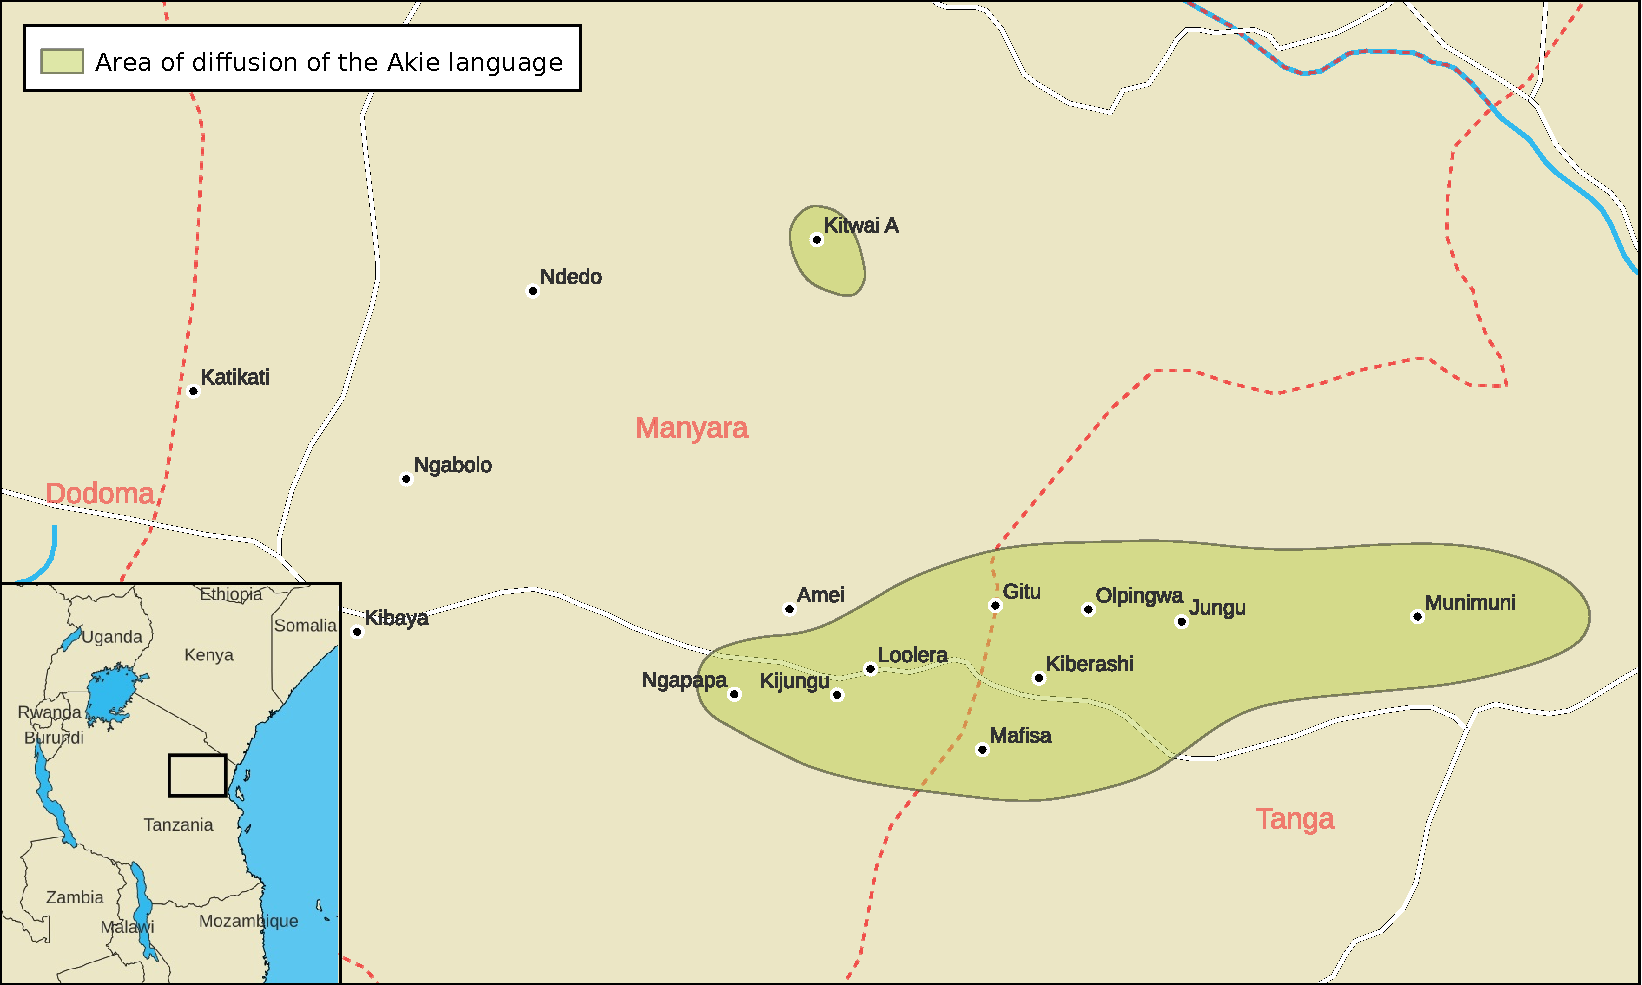
\includegraphics[width=\textwidth]{figures/akie_language_map.pdf}
    \caption{Distribution of the Akie language.\label{fig:legere:1}}
    % the Akie community and an estimate of the speaker number}
\end{figure}

\section{The Akie documentation project}\label{sec:legere:2}

The texts presented below form an integral part of the work on documenting the Akie language. Initially (from 2009 to 2011) the Akie documentation took place within the framework of the Languages of Tanzania (LoT) Project (Gothenburg University-University of Dar es Salaam, Department of Foreign Languages and Linguistics cooperation; Gothenburg coordinator K. Legère) funded by the Swedish International Development Cooperation Agency (SIDA). Subsequently in 2012, the Volkswagen Foundation assumed funding of the Akie documentation as part of the Documentation of Endangered Languages (\textit{Dokumentation Bedrohter Sprachen}, DoBeS) initiative, by way of two separate studies, namely “Akie in Tanzania: Documenting a critically endangered language” (2012 to 2015) and “Akie in Tanzania: Updating the documentation of a critically endangered language” (2017 to 2019). The fieldwork results, which are derived from the aforementioned 60 settlements in the Manyara and Tanga Regions, culminated in a large collection of sound, video and text files as well as photographs, which have been deposited with the DoBeS Archive at the Max Planck Institute of Psycholinguistics in Nijmegen, The Netherlands. The DoBeS Archive forms part of the United Nations Educational, Scientific and Cultural Organisation (UNESCO) Memory of the World (MoW) Programme.\footnote{\url{https://archive.mpi.nl/islandora/object/lat}}

According to \citet[1]{HimmelmannEtAl2006}, “a language documentation is a lasting, multipurpose record of a language”, reflected in a wide range of multifaceted communicative events. Such documentation aims at providing “a comprehensive record of the linguistic practices characteristic of a given speech community” \citep[166]{Himmelmann1998}. The language documentation target is the collection of raw/primary data in recording sessions (both audio and visual) that encompass “as many and as broad a range as possible of communicative events” \citep[7]{HimmelmannEtAl2006} . It goes without saying that recordings as suggested here are the background of the Akie project against which the subsequent transcription, translation and linguistic analysis of the material take place.

The documentation approach is rather well-suited to making available a variety of linguistic elements from recorded communicative events, as e.g. narratives or interviews. In respect of the discourse marker (DM) discussed below, it is taken for granted that its elicitation would probably not be easy or even impossible, as any DM use is associated with the flow of discourse such as the spontaneous utterances during e.g. a conversation or a narrative. An interesting example of this kind of communicative event can be found in the recordings in Napilukunya, Ngababa and Losekito (Akie name of Gitu which is one of the main Akie settlements north of Kibirashi, see \figref{fig:legere:1}) during blessing/offering rituals that focus on  ancestors. Such a ceremony is referred to as \textit{kanaítaísɛ} in Akie (\textit{tambiko}\footnote{Described by \citet[449]{Johnson1939} as an “offering of oxen, … beer … made to propitiate the spirits of the dead”.} in Swahili). 

\section{Ancestral cult}\label{sec:legere:3}

\subsection{The socio-anthropological perspective}\label{sec:legere:3.1}

The audio and video material and its transcription in \sectref{sec:legere:3.2} provide an example of how the Akie, through their relationship to their ancestors, pay special attention to a specific social element as an essential factor of their identity. For the community as well as the individual, respect for the deceased and the maintenance of the associated tradition of involving the ancestors in essential social spheres play an important role. 

From a socio-anthropological point of view, \citet[364]{Ferraro2005} comments on the position of ancestors in the form of ancestor worship as follows:

\begin{itemize}
    \item It considers the welfare of the community;
    \item After death a person continues to interact and affects the lives of living descendants;
    \item Ancestors are guardians of the social and moral order;
    \item Ancestors are elevated to the status of ancestor ghosts, enjoying supernatural powers;
    \item Community practices/rituals designed to induce the ancestors to protect and to favor them, or at least not to harm living beings.
\end{itemize}

\noindent In addition, \citet[365]{Ferraro2005} points out: 

\begin{itemize}
    \item Ancestors punish individuals who violate behavioral norms.
\end{itemize}

\noindent This general overview also applies to the Akie community in up-country Tanzania, where the contact with the ancestors is being maintained. Aspects of the ancestral cult among the Akie is dealt with in the following subsection.

\subsection{The Akie community and ancestral worship}\label{sec:legere:3.2}
\begin{sloppypar}
Blessing/offering rituals called \textit{kanaítaísɛ} are an indispensable element of Akie tradition and culture. Such ceremonies are deeply rooted in the belief that the community must continuously be assured of their social values and harmony with their neighbors, nature, etc. During these ceremonies, \textit{Tororeita} (‘God’) and especially \textit{asííswe}\footnote{Singular \textit{asííswante}.} (‘ancestors’) are asked to bring peace, well-being, health, enough food and local beer to the community, while anger, intolerance and other offensive habits are rejected. Local beer is an important component of the ceremony itself and is also drunk directly afterwards. The ceremony is also performed before men go hunting, when someone is expected to travel, and when guests come to visit. In the latter case, the ceremony is held for visitors to familiarize them with the way the Akie community cultivates and respects traditional values.
\end{sloppypar}

Akie community members who were consulted emphasized that their ancestors play a substantial role in these ceremonies. They are said to be present whenever something significant happens, and they are always hungry and thirsty. There is also the belief that \textit{asííswe} turn into monsters if proper care is not taken of them. Thus, the main function of the ceremony is for the community to establish contact with this imaginary ancestral target group. 

In a videotaped conversation on 2016-02-25 in Mbeli\footnote{See the DoBeS/Akie video deposit: \texttt{2016\_02-25\_Mahojiano\_Mbeli\_Lesakat\_munimuni.mpeg},
\url{https://hdl.handle.net/1839/b41cca45-3c9b-4d78-b45f-7e650850cac4}.} with his fellow elder Nkoiseyyo,  Lesakat (L), who was one of the pillars of Akie culture and tradition, summarized the role of \textit{kanaítaísɛ} as follows:

% \begin{tabular}{| p{5cm}|  p{5cm}| }
%     \lsptoprule
%     L.: ... nan korio nen kanaitaisee, 
%         & L.: ... and now at the offering/blessing ritual,\\
%     inaitaise phi chaa eech, duo phaai. Kae ko 
%         &  adults, in particular elders, make it \\
%     khuumii, kiale. Keewa de duo 
%         & There is beer, it is bought. Thereafter \\
%     kiinaitaisa neen iyu. Leena yai de 
%         & the ceremony takes place.  Mainly news is \\
%     lokhoywe. 
%         & spread. \\
%     N.: Ko an lokhoywe chaa kimwaau?
%         & N.: This is which kind of news that is said? \\
%     L.: Kimwaau isoo de lokhoywe, 
%         & L.: News are just now told, because these \\
%     amu kiamchini phi chu kirkophek. 
%         & we tell people who have passed away. \\
%     Ko chichee kiamchin lokhoo, 
%         & And, we tell them about everything new \\
%     kiinaitaise. 
%         & when our ritual is made. \\
%     \lspbottomrule
% \end{tabular}
\ea
\begin{enumerate}
    \item[L.:]
    \begin{enumerate}
        \item[-]    ... nan korio nen kanaitaisee, inaitaise phi chaa eech, duo phaai.\\
                    `... and now at the offering/blessing ritual, adults, in particular elders, make it.'
        \item[-]    Kae ko khuumii, kiale.\\
                    `There is beer, it is bought.'
        \item[-]    Keewa de duo kiinaitaisa neen iyu.\\
                    `Thereafter the ceremony takes place.'
        \item[-]    Leena yai de lokhoywe.\\
                    `Mainly news is spread.'
    \end{enumerate}
    \item[N.:]
    \begin{enumerate}
        \item[-]    Ko an lokhoywe chaa kimwaau?\\
                    `This is which kind of news that is said?' 
    \end{enumerate}
    \item[L.:]
    \begin{enumerate}
        \item[-]    Kimwaau isoo de lokhoywe, amu kiamchini phi chu kirkophek. \\
                    `News is just now told, because this we tell people who have passed away.'
        \item[-]    Ko chichee kiamchin lokhoo, kiinaitaise. \\
                    `And, we tell them about everything new when our ritual is made.'
    \end{enumerate}
\end{enumerate}
\z

The ceremony usually takes place after sunset, i.e. at night. As mentioned above an obligatory prerequisite is beer (\textit{khúúmi}) in a container, such as a steel\slash aluminum drum or an old plastic Sadoline paint bucket. In the case of the ceremony in Napilukunya and Ngababa, community members brew beer from honey. As a rule, the ceremony is performed by at least one Akie elder (male or female) or someone familiar with the blessing/offering tradition. At the beginning of the ritual and thereafter at regular intervals, the performer dips \textit{ratiɲántɛ}\footnote{The Akie tree name is \textit{sangaratwe}. In Swahili the tree is \textit{mwegea} and its fruit \textit{yegea}.} (the fruit of the sausage tree, \textit{Kigelia africana}) in the beer, sucks in the liquid and then spits it out. After the ceremonial monologue all those who attend the ritual spend the evening together sharing food and drinks. The structure of the rituals and performance as well as the linguistic focus of the communicative event documentation  will be dealt with next.

\section{The  ancestral cult among the Akie and their linguistic constituents}\label{sec:legere:4}

Below are transcripts and idiomatic translations of three ceremonial discourses in Akie that were recorded audiovisually. A prominent feature of the texts is the respectful, polite way of addressing the ancestors. 

In the first text\footnote{The focus of text 1 and the following texts is on the presentation of a logical flow of words that is not interrupted by glossing. In response to a suggestion by one of the manuscript reviewers a short selection of glossed text is included in the appendix which is expected to demonstrate some elementary facts about Akie language structure.}  L as the performer introduces the guests from far away\footnote{Karsten Legère (KL), P. Mkwan’hembo (MK), L. Ole-Wanga.} (called “white giants”) to the \textit{asííswe}. Similarly, L welcomes the ancestors, inviting them to eat and to drink \textit{khúúmi}. They are asked to bless the community and clear the way for the ceremony, the participants, and others. The ancestors are finally expected to leave in peace.

The polite, respectful way of speaking to the imaginary target group of \textit{asííswe} is demonstrated in parts 1, 3 and 5 of text 1. When the recordings of this and other ceremonial monologues and their transcriptions were analyzed, it turned out that a specific linguistic element occupied a prominent position in this communicative event. This was the discourse marker (DM) \textit{hm} which, on the one hand, was traced in these parts as paying attention to the ancestors in attendance in general. On the other hand, in parts 2 and 4, several \textit{asííswe} were addressed by name. Thus, the text culminated in a sort of roll call,  where, as a token of confirming \textit{asííswe’s} presence, attention and acceptance, a mock “dialogue” was generated by L. In so doing, for those ancestors whose names were mentioned L imitated a fictitious \textit{hm} answer after the call. In this case, in an English roll call the DM \textit{hm} would be the equivalent of ‘yes’ (categorized as an answer particle), ‘here’ or ‘present’.

In general, at the offering/blessing ritual, the use of DM \textit{hm} is mainly associated  with the English affirmative sentence adverbial ‘yes’. When this lexical function of DM \textit{hm} was discussed with Akie resource persons such as L and Bahati Nguyaki (BN), both confirmed  this interpretation.\footnote{With respect to DMs including \textit{hm} see also \citet{HeineEtAl2017} and \citet[137--146]{KonigEtAl2015}. Apart from its role at the blessing/offering ceremony which is commented upon in this paper \textit{hm} is also used in narratives, where its function is the confirmation of the speaker’s wording and text content. Like \textit{ehee} in Swahili, DM \textit{hm} here encourages the narrator to go ahead. In this case, \citet[152]{HeineEtAl2017}  classify \textit{hm} as a connective DM expressing discourse continuity and introducing a new information unit, translated as ‘and then’.}\pagebreak

% \begin{table}
% \caption{Tex1 (Part 1): Performer = Nangiwinyo Lesakat}
% \begin{tabular}{| p{5cm} | p{5cm} | }
% \hline
% Part 1
% Ɔ́pwan nái, ɔɛ́ɛ́sien nen ɪʊ.
% Ɔɛ́ɛ́sien nái, s’ɔítɛ kɛɛn, ɔ́ɔ́pɛ. 
% Ɔ́pwan, ɔɛ́ɛ́sien nen ɪʊ, asííswɛ́, amʊ akílɛ ɗe:
% Kápwa tián chʊ lɛɛlách ii. Hm.
% Kɔ akwɛ́ i, kikúúrɛ amʊ ii. 
% Kɛ́ɛ́pwa, kɛ́ɛ́le:
% ɔmwáun ɗe lɔkoíywɛ tukul. 
% Hm. Kɔ́pwa kɔ́riekis. Hm.
% Koúp, anasínan, amíítwaaki tukuul. Hm. 
% Ɔ́ɛ́ɛ́sien nái, si ɔŋɛɛtítɛ, ɔ́ɔ́pɛ, hm, si ɔkóónu kurúɽta. Hm.
% Ɔítɛ kɛɛn akwɛ́, asííswɛ́, hm, ɪkaa laŋatáá ni. Hm. 
% Ɔmáátɛɛn asíísi. Hm.
% Amu kɔ akwɛ́ɛ́, kakípwan kɛ́ɛ́saam kuutii. Hm.
% Akɛ́ɛ́saam kíí ya kimáchɛ. Hm.
% Kɔ́wa kɔ́puɽ íyya kɛnkɛɛni. Hm.
% Am(u) kimáchɛ ɗe, kɛ́ɛ́taakak pɔ́ɔ́rwɛ. Hm. 
% Makimáchɛ ɗe isóo achɛɛ, hm, amóo píí ɗe chaa ŋɛ́ɛ́tin iyya pa raai, Hm.
% Ɔ́pwan, ɔɛ́ɛ́sien, si ɔŋɛ́titɛ.
% Ɔ́ɔ́pɛ, s’ɔkoonɛ́ɛ́ch kurúɽta, s’ɔpaipái sɛkɛ́rí. Hm.
% Ɔ́ítɛ kátóo, ɔítɛ ŋwénááni. Hm.
% Ɔ́kaachi ŋɛ́ɛ́taa kɔ́pa, hm, nen sííŋo-wínta. Hm.
% Ɔ́ítɛ nai kɛɛn ɔɔkwɛ́ɛ́. Hm. Lalei. Hm. 
% Kɔ leenai kimwaayɛ́. Hm. 
% Kɔ chaa íra lɔkóiywe, hm, ika yaa kiyá i, hm, Ámʊ arkéépwa.  & 

% Part 1
% Come now, drink here. 
% Drink now, so that you may move, leave. 
% Come, drink here, spirits [ancestors], because we have just said: 
% White giants have come. Hm.  
% It is you who have been called for this. 
% They came to say: 
% Just tell us all words. Hm. 
% They came to brew beer. Hm.
% Folks, they brought in all the food. Hm.
% Drink now so you may get out and go, hm, so as to give us health. Hm.
% Move yourselves out, ancestors, hm, of tonight. Hm. 
% Follow this sun. Hm. 
% Because it is you whom we come to ask for the language. Hm.
% We ask for what we want. Hm. 
% It became stalled in one place. Hm. 
% Because we just want to see your bodies. Hm. 
% We do not want just now, hm, because we are not just people who are from the open place. Hm. 
% Come, drink, and leave. 
% Go as to give us health, to guide the soul straight. Hm. 
% Move the thorns, move the holes. Hm. 
% Give men a chance to go, hm, in comfort. Hm. 
% Move yourselves now. Hm. Look. Hm. 
% This is what we are saying. Hm. 
% These are words, hm, of this coun-try, hm, because they [guests] have come.\\
% \hline

% \end{tabular}
% \end{table}

\ea Tex1: Part 1 (Performer = Nangiwinyo Lesakat)\largerpage
    \ea    Ɔ́pwan nái, ɔɛ́ɛ́sien nen ɪʊ.\\
            `Come now, drink here.'
    \ex     Ɔɛ́ɛ́sien nái, s’ɔítɛ kɛɛn, ɔ́ɔ́pɛ. \\
            `Drink now, so that you may move, leave.'
    \ex     Ɔ́pwan, ɔɛ́ɛ́sien nen ɪʊ, asííswɛ́, amʊ akílɛ ɗe:\\
            `Come, drink here, spirits [ancestors], because we have just said:'
    \ex     Kápwa tián chʊ lɛɛlách ii. Hm.\\
            `White giants have come. Hm.' 
    \ex     Kɔ akwɛ́ i, kikúúrɛ amʊ ii. \\
            `It is you who have been called for this.'
    \ex     Kɛ́ɛ́pwa, kɛ́ɛ́le:\\
            `They came to say:'
    \ex     ɔmwáun ɗe lɔkoíywɛ tukul. Hm. \\
            `Just tell us all words. Hm.'
    \ex     Kɔ́pwa kɔ́riekis. Hm.\\
            `They came to brew beer. Hm.'
    \ex     Koúp, anasínan, amíítwaaki tukuul. Hm. \\
            `Folks, they brought in all the food. Hm.'
    \ex     Ɔ́ɛ́ɛ́sien nái, si ɔŋɛɛtítɛ, ɔ́ɔ́pɛ, hm, si ɔkóónu kurúɽta. Hm.\\
            `Drink now so you may get out and go, hm, so as to give us health. Hm.'
    \ex     Ɔítɛ kɛɛn akwɛ́, asííswɛ́, hm, ɪkaa laŋatáá ni. Hm. \\
            `Move yourselves out, ancestors, hm, of tonight. Hm.'
    \ex     Ɔmáátɛɛn asíísi. Hm.\\
            `Follow this sun. Hm.'
    \ex     Amu kɔ akwɛ́ɛ́, kakípwan kɛ́ɛ́saam kuutii. Hm.\\
            `Because it is you whom we come to ask for the language. Hm.'
    \ex     Akɛ́ɛ́saam kíí ya kimáchɛ. Hm.\\
            `We ask for what we want. Hm.'
    \ex     Kɔ́wa kɔ́puɽ íyya kɛnkɛɛni. Hm.\\
            `It became stalled in one place. Hm.'
    \ex     Am(u) kimáchɛ ɗe, kɛ́ɛ́taakak pɔ́ɔ́rwɛ. Hm.\\
            `Because we just want to see your bodies. Hm.'
    \ex     Makimáchɛ ɗe isóo achɛɛ, hm, amóo píí ɗe chaa ŋɛ́ɛ́tin iyya pa raai, Hm.\\
            `We do not want just now, hm, because we are not just people who are from the open place. Hm.'
    \ex     Ɔ́pwan, ɔɛ́ɛ́sien, si ɔŋɛ́titɛ.\\
            `Come, drink, and leave.'
    \ex     Ɔ́ɔ́pɛ, s’ɔkoonɛ́ɛ́ch kurúɽta, s’ɔpaipái sɛkɛ́rí. Hm.\\
            `Go as to give us health, to guide the soul straight. Hm.'
    \ex     Ɔ́ítɛ kátóo, ɔítɛ ŋwénááni. Hm.\\
            `Move the thorns, move the holes. Hm.'
    \ex     Ɔ́kaachi ŋɛ́ɛ́taa kɔ́pa, hm, nen sííŋo-wínta. Hm.\\
            `Give men a chance to go, hm, in comfort. Hm.'
    \ex     Ɔ́ítɛ nai kɛɛn ɔɔkwɛ́ɛ́. Hm. Lalei. Hm.\\
            `Move yourselves now. Hm. Look. Hm.'
    \ex     Kɔ leenai kimwaayɛ́. Hm.\\
            `This is what we are saying. Hm.'
    \ex     Kɔ chaa íra lɔkóiywe, hm, ika yaa kiyá i, hm, Ámʊ arkéépwa.\\
            `These are words, hm, of this country, hm, because they [guests] have come.'
    \z


% \begin{table}{!ht}
% \caption{Text 1: Part 2 to Part 5} (Performer = Nangiwinyo Lesakat)
% \begin{tabular}{| p{5cm} | p{5cm}| }
% \hline
% Part 2 & Part 2 \\
% Ɔ́pwan nái, pháápha, hm, pháápha Sapáí, hm, Lɔitiakí, hm, Kaíyakaí, hm, Namaiyai, hm. & 
% Come now, Father, hm, Father Sapai, hm, Loitiaki, hm, Kaiyakai, hm, Namaiyai, hm.\\
% \hline
% Part 3 &  Part 3 \\
% Ɔ́pwan nái, ɔpasúún kɛɛn tukuul, hm, s’ɔítɛ kɛɛn, hm, si ɔkoonɛ́ch ɗe ɲɛ́ɛ́ kurúɽta. Hm.  &
% Come now, gather yourselves all, hm, so that may move, hm, so that you can  give us health now. Hm.\\
%  \hline
%  Part 4 & Part 4 \\
%  Amóó, hm, Moisári, hm, Naiyasoi, hm. 
%  Ɔ́pwan nái, hm, Lɔlóísya, hm, Tóótɔ, hm, Lɛmɔ́na, hm, Ngusɛrɔ́ɔ, hm.
%  & 
%  Mother, hm, Moisari, hm, Naiyasoi, hm. 
%  Come now, hm, Loloisya, hm, Tooto, hm, Lemona, hm, Nguseroo, hm. \\
%  \hline
%  Part 5 & Part 5 \\
%  Ɔpasúún nái kɛɛn tukuul, hm, 
% si ɔítɛ kɛɛn ɔ́ɔ́kwɛ, hm,
% si ɔkóónu kurúɽta, hm, si ɔítɛ kɛɛn, 
% si ɔkaachí kɔ́ɔ́ɲɛ chʊʊ, 
% kolasiya, hm. Leláa kulɔ, 
% s’áási ɗe ɲɛ́ɛ́ íya apʊ́nɛ, na alapátii, hm 
% am(ʊ) kakílɛ ɗe, arkoyáii, s’áási ɗe ɲɛ́ɛ́ am kakílɛ ɗe, arkoyáii ólta, arkóe na kiparé phii, hm.
% & 
% Gather now yourselves all, hm,
% so that you can move out, hm,
% so that you may give health, hm, so that you can leave, so that you may give me my eyes, they will heal, hm. You folks,
% so that I find a way to pass and run, hm, 
% because it was just said, the words are broken, there are people who are being killed, hm.\\
% \hline
 

% \end{tabular}
% \end{table}

\ex   Part 2\\\largerpage[1]
      Ɔ́pwan nái, pháápha, hm, pháápha Sapáí, hm, Lɔitiakí, hm, Kaíyakaí, hm, Namaiyai, hm.\\
      `Come now, Father, hm, Father Sapai, hm, Loitiaki, hm, Kaiyakai, hm, Namaiyai, hm.'
\ex   Part 3\\
      Ɔ́pwan nái, ɔpasúún kɛɛn tukuul, hm, s’ɔítɛ kɛɛn, hm, si ɔkoonɛ́ch ɗe ɲɛ́ɛ́ kurúɽta. Hm.\\
      `Come now, gather yourselves all, hm, so that you may move, hm, so that you can  give us health now. Hm.'
\ex   Part 4
      \ea Amóó, hm, Moisári, hm, Naiyasoi, hm.\\
          `Mother, hm, Moisari, hm, Naiyasoi, hm.'
      \ex Ɔ́pwan nái, hm, Lɔlóísya, hm, Tóótɔ, hm, Lɛmɔ́na, hm, Ngusɛrɔ́ɔ, hm.\\
          `Come now, hm, Loloisya, hm, Tooto, hm, Lemona, hm, Nguseroo, hm.'
      \z
\ex   Part 5
    \ea Ɔpasúún nái kɛɛn tukuul, hm, si ɔítɛ kɛɛn ɔ́ɔ́kwɛ, hm, si ɔkóónu kurúɽta, hm, si ɔítɛ kɛɛn, si ɔkaachí kɔ́ɔ́ɲɛ chʊʊ, kolasiya, hm.\\
        `Gather now yourselves all, hm, so that you can move out, hm, so that you may give health, hm, so that you can leave, so that you may give me my eyes, they will heal, hm.'
    \ex Leláa kulɔ, s’áási ɗe ɲɛ́ɛ́ íya apʊ́nɛ, na alapátii, hm am(ʊ) kakílɛ ɗe, arkoyáii, s’áási ɗe ɲɛ́ɛ́ am kakílɛ ɗe, arkoyáii ólta, arkóe na kiparé phii, hm.\\
        `You folks, so that I find a way to pass and run, hm, because it was just said, the words are broken, there are people who are being killed, hm.'
    \z
\z

The structure of the 2010 \textit{kanaítaísɛ }recording (text 2 below) is similar to that of text 1 above. In this ceremony, first a female and then a male elder take part. In part 1, N Muringa (M) explains that guests who want to know more about the Ngababa Akie community and the Akie language have arrived in Ngababa. Accordingly, the Akie community members in this village organized various events for their visitors, including a blessing/offering ritual which took place on 2010-08-04. 
In text 2, part 1, M produces \textit{hm} three times. In text 2, part 2, L follows the pattern that he had demonstrated in his 2009 performance above (text 1).

% \begin{table}
% \caption{Text 2: Part 1 (Performer = Nekitoliya Muringa)}
% \begin{tabular}{| p{5cm} | p{5cm} | }
% \hline
% Part 1 & Part 1 \\

% Iki yai khuumi, phaapha, akipwaan nai iyaa iinte phaapha Teeye ai Patina. 
% Ichi khuumi opwaan, oeesien. Hm. Ko phii chaa ko tayee chu chaa kapwa, kolei:
% Opwaan, nyon, olaleech akɛɛche. 
% Ko makiweche de akeeche, amu kipare:
% “Kosii okaseech olaa kiintee, amu arkeeyoosiitu de, kiisyeptooseii.”
% Ko chaa yai, phaapha, hm, ako Lepatoi, hm.
% &
% This beer now, Father, we have just come where you are, Father Teeye and Patina. These beers, come and drink them, hm. There are these guests who have come, saying:
% Come [pl.], come [sg.], look at us. 
% And we do not reject them, for we say:
% “Let them understand where we are, just being old, still living.”
% It is this now, Father, hm, Lepatoi people, hm.\\
% \hline

% \end{tabular}
% \end{table}

\ea Text 2: Part 1 (Performer = Nekitoliya Muringa)
        \ea    Iki yai khuumi, phaapha, akipwaan nai iyaa iinte phaapha Teeye ai Patina.\\ 
                `This beer now, Father, we have just come where you are, Father Teeye and Patina.'
        \ex    Ichi khuumi opwaan, oeesien. Hm. Ko phii chaa ko tayee chu chaa kapwa, kolei:\\
                `These beers, come and drink them, hm. There are these guests who have come, saying:'
        \ex    Opwaan, nyon, olaleech akɛɛche.\\
                `Come [pl.], come [sg.], look at us.'
        \ex    Ko makiweche de akeeche, amu kipare:\\
                `And we do not reject them, for we say:'
        \ex    “Kosii okaseech olaa kiintee, amu arkeeyoosiitu de, kiisyeptooseii.”\\
                `“Let them understand where we are, just being old, still living.”'
        \ex    Ko chaa yai, phaapha, hm, ako Lepatoi, hm.\\
                `It is this now, Father, hm, Lepatoi people, hm.'
  \z
\z


The part 1 text continues, but is not included here, because no DM hm is used. The same applies to the introductory section of text 2, part 2, which is skipped, for no \textit{hm} is applied.

% \begin{table}
% \caption{Text 2 (Part 2)
% (Performer = Nangiwinyo Lesakat)}
% \begin{tabular}{| p{5cm} | p{5cm} | }
% \hline
% Part 2 & Part 2 \\
% ... Ko akwe; kikuure. 
% Opwan nai de duoi. 
% Ophasuun keen, asiiswe, hm. 
% Phaapha, hm, Saphai, hm, kos’oopwan nai de duo. 
% Ophasuun keen, hm. 
% Loitiaki Kaiyakai, Oltungu, opwan nai, ophasuun keen tukuul. 
% Kaiyakai, opwan nai, hm, nen iyu. 
% Hm. 
% Taiko, hm, Kisema, hm, Alapuopuo, hm, Nguseroo, hm & 
% ... It is you; you are called. 
% Just come now. 
% Assemble yourselves, ancestors, hm. 
% Father, hm, Saphai, hm, so that you (all) just come. 
% Assemble yourselves, hm. 
% Loitiaki Kaiyakai, Oltungu, just come, assemble yourselves all. 
% Kaiyaikai, come now, hm, over here. 
% Hm. 
% Taiko, hm, Kisema, hm, Alapuopuo, hm, Nguseroo, hm. \\
% \hline
% \end{tabular}
% \end{table}

\ea    Part 2 (Performer = Nangiwinyo Lesakat)
        \ea   ... Ko akwe; kikuure.\\
              `... It is you; you are called.'
        \ex    Opwan nai de duoi.\\
               `Just come now.'
        \ex    Ophasuun keen, asiiswe, hm.\\
               `Assemble yourselves, ancestors, hm.'
        \ex    Phaapha, hm, Saphai, hm, kos’oopwan nai de duo.\\
               `Father, hm, Saphai, hm, so that you (all) just come.'
        \ex    Ophasuun keen, hm.\\
               `Assemble yourselves, hm.'
        \ex    Loitiaki Kaiyakai, Oltungu, opwan nai, ophasuun keen tukuul.\\
               `Father, hm, Saphai, hm, so that you (all) just come.'
        \ex    Kaiyakai, opwan nai, hm, nen iyu. Hm.\\
               `Assemble yourselves, hm. Hm.'
        \ex    Taiko, hm, Kisema, hm, Alapuopuo, hm, Nguseroo, hm.\\
              `Taiko, hm, Kisema, hm, Alapuopuo, hm, Nguseroo, hm.'
    \z
\z

Altogether, L produced the DM \textit{hm} at least 21 times. It occurred 10 times in what could be interpreted as a roll call of the ancestors. When L addressed the ancestors in a more general way (not calling them by their names), the DM was used another 11 times.
Another blessing/offering ritual was recorded on 2013-01-31 by Christa König and Bernd Heine in Losikito (Gitu). Text 3 below is an extract from their transcript of a ceremony performed by Nkauli Samakuya (NS). In NS’s speech, the DM hm is even more widely used (namely a total of 58 times) than in texts 1 or 2 above. Here are samples of this 2013 material.

% \begin{table}
% \caption{Text 3 (Performer = Nkauli Samakuya)}
% \begin{tabular}{ | p{5cm} | p{5cm}| }
% \hline
% 1/61 & 1/61 \\
% Óeesien, hm, ásiiswé ikáá kíyaí pa Mókiri, hm.
%  &
%  Drink, hm, ancestors of this country of Mokiri, hm \\
%  \hline
%  1/65 & 1/65 \\
%   Keleí: Hm, óyumuyumun náá kɛn, hm, áko Kɪkɛ́kɔ, hm.
% & 
% We say: Hm, gather yourselves, hm, Kikeko people, hm.
% \\
% \hline
% 1/66 & 1/66 \\
% Ɛlá, kɔlɔ, hm, ichi ɗeí kaai táá Kisíko, hm, kaai táá Kisíko, hm. 
% Akó Injulu, hm, ako Taaye, hm, lɛláá, ako Lesikeí, hm. 
% ɛláá, kɔlɔ, hm, akó Párleti, hm, lɛlaa, kɔlɔ, hm. 
% & 
% Folks, indeed, hm, this [is] now the town of Kisiko, hm, the town of Kisiko, hm. 
% Injulu people, hm, Taaye people, hm, Lesikai people, hm, Parleti people, hm, folks, indeed, hm.\\
% \hline

% \end{tabular}
% \end{table}

\ea Text 3 (Performer = Nkauli Samakuya)
    \ea    Óeesien, hm, ásiiswé ikáá kíyaí pa Mókiri, hm.\hfill [1/61]\\
            `Drink, hm, ancestors of this country of Mokiri, hm.'
    \ex    Keleí: Hm, óyumuyumun náá kɛn, hm, áko Kɪkɛ́kɔ, hm.\hfill [1/65]\\
            `We say: Hm, gather yourselves, hm, Kikeko people, hm.'
    \ex    Ɛlá, kɔlɔ, hm, ichi ɗeí kaai táá Kisíko, hm, kaai táá Kisíko, hm.\hfill [1/66]\\
            `Folks, indeed, hm, this [is] now the town of Kisiko, hm, the town of Kisiko, hm.'
    \ex    Akó Injulu, hm, ako Taaye, hm, lɛláá, ako Lesikeí, hm.\\
            `Injulu people, hm, Taaye people, hm, Lesikai people, hm.'
    \ex    ɛláá, kɔlɔ, hm, akó Párleti, hm, lɛlaa, kɔlɔ, hm.\\
           `hm, Parleti people, hm, folks, indeed, hm.'
    \z
\z

The texts produced by even experienced Akie speakers such as Papalai Kalisya on 2013-10-30 (in a short blessing/offering ceremony of two minutes) and earlier B. Nkoiseyyo together with Nkúyáki Rokina in Losekito (Gitu) on 2013-01-31 (more elaborate and longer, but very general) are short of the mock dialogue with the community’s ancestors. In this respect, the names of the ancestors are no longer quoted, probably because they may not be known any more. Consequently, the emphasis of other more recent blessing ceremonies witnessed during fieldwork has now shifted to the prevailing situation and its hardships for the Akie.

\section{To sum up}\label{sec:legere:5}

This paper has dealt with some aspects of the documentation of the Akie language using the example of ceremonial discourse as part of the ancestral cult.  In this respect the function of the DM \textit{hm} was discussed which, in the texts included here, is associated with blessing/offering rituals that have been recorded since 2009 in Akie community settlements. 

The text samples selected above demonstrate how the ceremonies emphasize maintaining and consolidating a ritual relationship with the community’s ancestors. The respect bestowed on deceased members of the community and – from the perspective of the living – the unilateral contact with them forms a substantial pillar of Akie traditions and heritage.

The discourse strategy in \textit{kanaítaísɛ} employs two principal ways of addressing ancestors, who are expected to take note of what they are being told. The first method is more general, speaking to them without any name, while the second entails appealing to them directly by name. The ancestors are deemed to be responding to being addressed in these ways. For example, the performer of the ceremony utters on behalf of the \textit{asííswe} a short mock response by way of the DM \textit{hm}. When the ancestors are appealed to directly by name in a type of roll call, the mock response \textit{hm} corresponds with ‘here’, ‘yes’ or ‘okay’ in English, and indicates that somebody is present. In terms of the ceremony “dialogue” content per se, not only are the ancestors invited to \textit{kanaítaísɛ} to drink beer and to eat, they are also requested to pave the way for the arrival of guests or latecomers, ease the passage for community members that are leaving, and bestow peace and well-being on the Akie people.

The material presented here is a symbol of the Akie language versatility that however, is becoming more and more rare. Both N Lesakat and N Muringa, who were known and respected as guardians of the language (displaying sophisticated language use, rich in its vocabulary and grammatical structures), Akie history, traditions and other facets of Akie life  have passed away. 

Another aspect of continuing to uphold Akie traditions and heritage has to do with maintaining \textit{kanaítaísɛ} in view of the small number of Akie-speaking persons who may be exposed to this and other communicative events. Given that many Akie people live scattered and isolated in small settlements far from each other, it is often not possible to gather enough participants to enact any ritual. That’s why ceremonies can only be practiced in a few places such as Losekito and Napilukunya, where a reasonable number of Akie speakers can still be found.

In conclusion, therefore, the future of the Akie blessing/offering ritual in the traditional manner – or even in a modern version which was referred to above -- is bleak. Taking this situation into account, the assessment of ongoing language change, attrition and loss as portrayed in this paper with respect to \textit{kanaítaísɛ} as one of the pillars of the hunter-gatherer Akie community serves to corroborate once again Akie’s status as a critically endangered Tanzanian language.


\section*{Abbreviations}

\begin{multicols}{3}
\begin{tabbing}
\textsc{coll}\hspace{1ex}\= Collective plural\kill
\textsc{a} \> Accusative\\
\textsc{ad} \> Accusative \\ \> demonstrative\\
\textsc{ap} \>  Antipassive\\
\textsc{coll} \> Collective plural\\
\textsc{cop} \> Copula\\
\textsc{D} \> Distal\\
\textsc{dm} \> Discourse marker\\ 
\textsc{excl} \> Exclamation\\ 
\textsc{gen} \> Genitive\\ 
\textsc{imp} \> Imperative\\ 
\textsc{loc} \> Locative\\
\textsc{pl} \> Plural\\
\textsc{pr} \> Proximal\\
\textsc{prep}  \> Preposition\\
\textsc{rel} \> Relative marker\\ 
\textsc{rfl} \> Reflexive\\ 
\textsc{s} \> Subjunctive\\
\textsc{sg} \> Singular\\
\textsc{ven} \> Ventive
\end{tabbing}
\end{multicols}

\section*{Acknowledgments}
The authors hereby express their gratitude to the Volkswagen Foundation, which has generously supported and financed the extensive activities of two documentation projects since 2012. Similarly, the SIDA support for KL's field work in 2009/2010 is acknowledged with thanks. In this regard, the University of Dar es Salaam has authorized KL's Endangered Languages in Tanzania research project (as part of LoT cooperation) and granted permission for the field research under the Akie (Ref. No.: AB3/3(B)). There was also exemplary support from regional authorities (Tanga and Manyara). At the grassroots level the cooperation with Akie language experts, speakers and other Akie community members was excellent. The commitment shown by the local resource persons and Tanzanian assistants, as well as their initiative have left an indelible impression. A pre-final version of this paper was checked language-wise by Ms. Sandra Fitchat (Swakopmund, Namibia). Her language revision and paper comments were substantial and stimulating. However, the views expressed in this paper are entirely those of the authors. 
Ahsanteni sana -- many thanks to all.

\section*{Appendix}

\ea
    \ea[]{
    \gll    ó ee-sie-n hḿ ásiiswê ikáá kíya-í pa mókiri \textit{hḿ}\\
    \textsc{2pl} drink.\textsc{s-ap-imp} hm ancestors.\textsc{a} \textsc{gen} land.\textsc{ad.pr.sg} \textsc{loc.gen} Mokiri.\textsc{a} hm \\
	\glt    `You should drink, \textit{hm}, ancestors of this country of Mokiri, \textit{hm}.' (1/61)}
	\ex[]{
    \gll    Akiye ká mókiri \textit{hḿ}  ǹte ɗé iyu\\
    Akiye.\textsc{a} \textsc{gen} Mokiri.\textsc{a} hm exist \textsc{dm} here\\
    \glt    `Akiye of Mokiri, \textit{hm}, exist here.' (1/62)}
	\ex[]{
 	\gll    \textit{hḿ} kɔ nɪnyɛ ɗé ni kíí ntei-yak nen iyû nkúyaki \textit{hm}\\
    hm \textsc{cop} \textsc{3.sg.a} \textsc{dm} \textsc{rel.sg} \textsc{1.pl} be.together \textsc{prep} here Nkuyaki hm\\
    \glt  `\textit{Hm}, it is him who we were all together with here in Nkuyaki, \textit{hm}.' (1/63)}
	\ex[]{
    \gll inkúyaki ɗe ko inkúyaki ɗe ni \textit{hḿ}\\
    Inkuyaki \textsc{dm} \textsc{cop} Inkuyaki.\textsc{a} \textsc{dm} \textsc{d.pr.sg} hm\\
     \glt   `It is Inkuyaki there, \textit{hm}.' (1/64)}
	\ex[]{
    \gll    ke leí \textit{hḿ} ó yumuyumu-n náá kɛn \textit{hḿ} áko kɪkɛ́kɔ \textit{hḿ} \\
    \textsc{1.pl} say hm \textsc{2.pl} gather.\textsc{s-ven-imp} \textsc{rel.sg} \textsc{rfl} hm \textsc{coll.a} Kikeko hm\\
    \glt    `We say: \textit{Hm}. You who are Kikeko folks, \textit{hm}, should gather all together.' (1/65)}
	\ex[]{
    \gll ɛlá kɔlɔ  \textit{hḿ} iciɗeí kaai táá kisíko \textit{hḿ} kai táá kisíko \textit{hḿ}\\
    folks \textsc{excl} hm here town.\textsc{a} \textsc{gen} Kisiko.\textsc{a} hm town.\textsc{a} \textsc{gen} Kisiko.\textsc{a} hm\\
    \glt    `Folks, \textit{hm}, here the town of Kisiko, \textit{hm}.' (x2) (1/66)}
    \z
\z

\printbibliography[heading=subbibliography,notkeyword=this]

\end{document}
